\label{chap:introduction}

%Cite me: Architectural Aspects of Self-Aware and Self-Expressive Computing Systems: From Psychology to Engineering~\cite{LewisEtAl2015}. %It can be a good paper to cite in your intro, to give a broader sense of what people think when we mention self-awareness, then you can narrow the focus in your contributions and in the background.

%Cite me in discussion of self-awareness: Revisiting Goal-Oriented Models for Self-Aware Systems-of-Systems\cite{CavalcanteEtAl2015}.

%Cite me in discussion of self-awareness: Self-Aware and Self-Expressive Systems~\cite{TorresenEtAl2015}.

%Cite me in discussion of self-awareness: Self-aware architecture to support partial control of emergent behavior~\cite{MotusEtAl2012}.

As we move toward an exascale future with ever expanding capacities in terms of both cores and resources, we have reached a point in computing where current execution paradigms will no-longer suffice. High performance computing systems have begun to approach a point where the ever growing multiplicity of transistor counts and components is not sustainable in terms of energy consumption. It has been said that at the current rates, extrapolated into the future, that an exascale computer system would consume over 1.5~GW of power~\cite{Green500Year3}. These ever expanding power requirements necessarily result in the need for a fundamental and radical shift in terms of programmability and adaptation. We believe that systems will need to become hierarchically introspective and self-aware to be able to adapt to these steep performance and energy requirements.

There are number of key facets that need to be addressed to enable a truly introspective and self-aware system capable of performing well and efficiently. The first is that a form of co-design needs to occur in terms of hardware and software. Exascale hardware needs to support a number of integral features to enable controlling system software to monitor and adapt to the current system state and any requirements passed to it in the form of power or performance. In broad terms, there will need to be some form of an observe-decide-act (ODA) loop to monitor, make decisions, and to control both the hardware and software aspects of a system. The second is that the system needs to be capable of adapting for power and performance while at the same time maintaining correct and reliable operation. It is key to recognize that these conflicting goals form a basis for a multi-variable problem which will be further complicated by the need to run multiple programs on a system with thousands of components. As highlighted in my prior work on self-aware systems for exascale architectures~\cite{Landwehr2014}, there is an open question on how to self-adjust and to meet these goals. The third facet is to propose a hierarchical method to control the system using ODA loops in conjunction with the co-designed hardware and software features available within the system.

\begin{figure}[htb!]
    \centering
    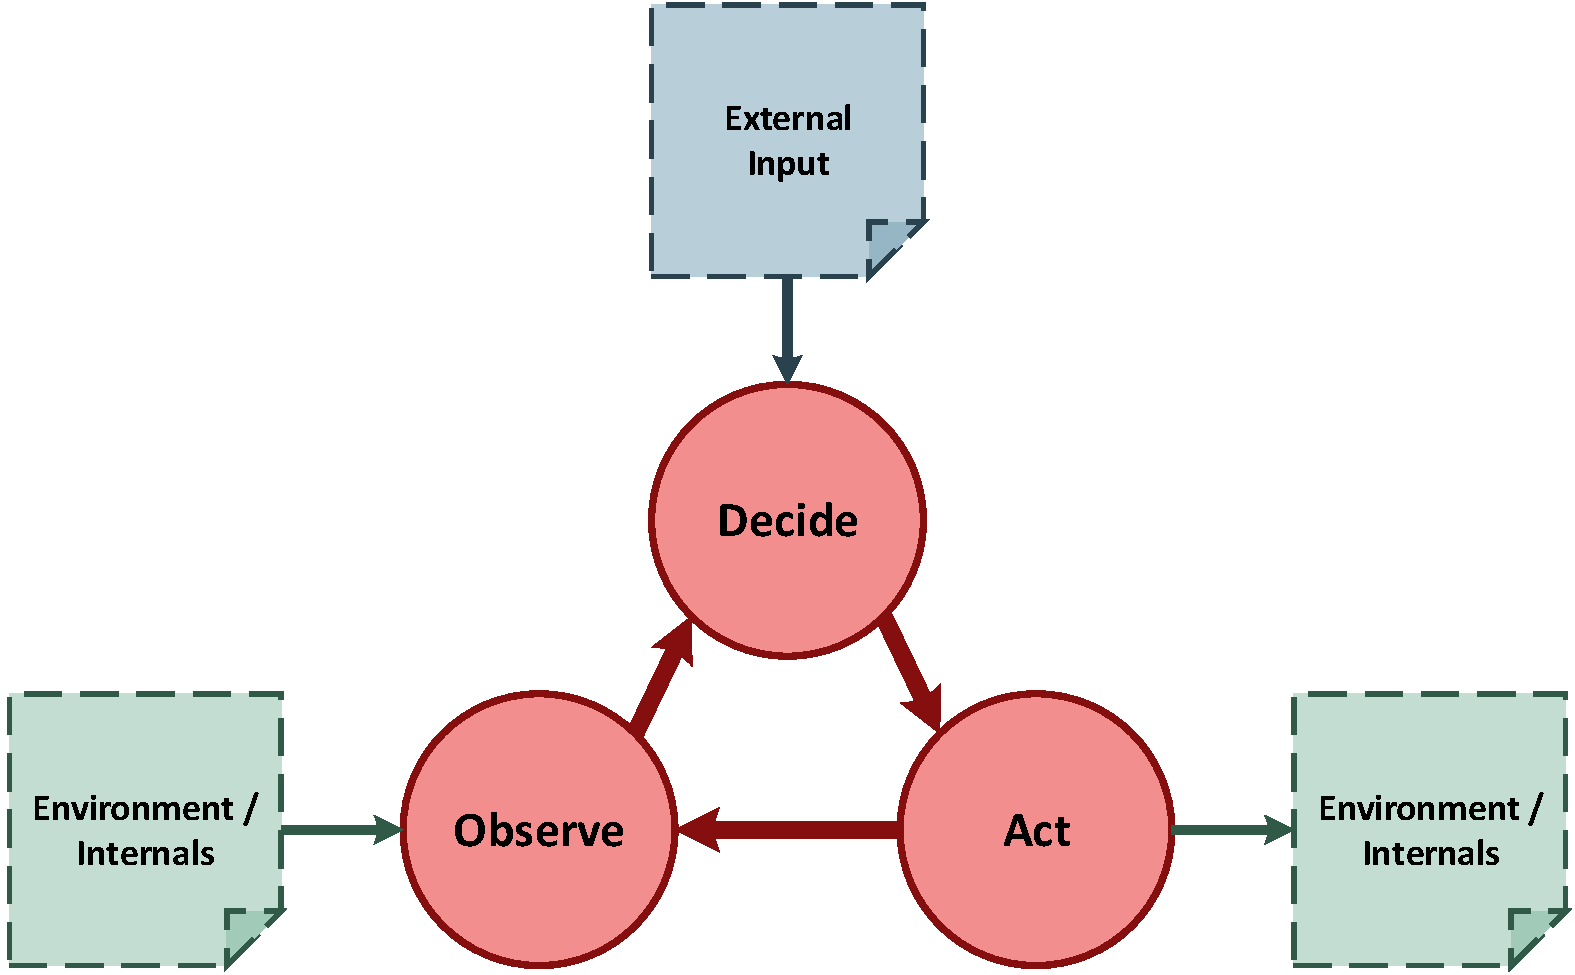
\includegraphics[width=0.7\textwidth]{Fig/ODA_loop_general.pdf}
    \caption[Generalized ODA Loop]{A generalized ODA loop consisting of observe, decide, and act stages.}
    \label{fig:ODA-generic}
\end{figure}

In more detail, adaptation will need to occur using ODA loops as shown in Figure~\ref{fig:ODA-generic}. These are a type of self-feedback loop consisting of three stages where each stage feeds back to another stage in the process. The observe stage collects information from the system environment. The decide stage is where decisions are made based upon observed information and possibly some form of external input. In this context, a decision is answering the question of \textit{what} to do in the system not \textit{how} to achieve the objective. The act stage translates a decision into a set of actions which are then committed by adjusting some form of actuators. This stage answers the question of \textit{how} to adapt. For instance, this could be to adjust core frequencies or some combination of actuators or knobs.

This thesis serves to discuss many facets involved with these aspects of exascale systems. The detailed discussion includes an abstract Target Exascale Architecture (TEA) representative of the trends seen in the move toward exascale computing, as well as, the challenges present within self-aware and adaptive exascale systems. As exascale systems will require specific features to enable adaptation, an exhaustive discussion of hardware and software requirements is detailed within. Additionally, an experimental simulation framework for exascale architectures incorporating many of the hardware/software requirements is implemented and tested to demonstrate adaptive control policies. This framework uses hierarchical distributed control to implement a self-adaptive power management system. Finally, hierarchical adaptive control policies are evaluated using a number of workloads, and a number of conclusions regarding self-adaptive exascale systems are made.

The thesis is organized as follows: Chapter~\ref{chap:background} defines the abstract Target Exascale Architecture. Chapter~\ref{chap:problem_formulation} discusses the open questions toward self-aware exascale systems, and a solution methodology toward answering those questions. Chapter~\ref{chap:requirements} discusses the hardware/software requirements for a self-adaptive exascale system.  Chapter~\ref{chap:framework} discusses our simulation frame and the various models it implements. Chapter \ref{chap:results} discusses the experimental results obtained using the framework. Chapter~\ref{chap:related_work} discusses various state of the art works on adaptation, as well as, the limitations. Chapter~\ref{chap:conclusion} provides concluding discussion.

